%%====Preamble====
\documentclass[12pt]{article}\usepackage{graphicx, color}
%% maxwidth is the original width if it is less than linewidth
%% otherwise use linewidth (to make sure the graphics do not exceed the margin)
\makeatletter
\def\maxwidth{ %
  \ifdim\Gin@nat@width>\linewidth
    \linewidth
  \else
    \Gin@nat@width
  \fi
}
\makeatother

\IfFileExists{upquote.sty}{\usepackage{upquote}}{}
\definecolor{fgcolor}{rgb}{0.2, 0.2, 0.2}
\newcommand{\hlnumber}[1]{\textcolor[rgb]{0,0,0}{#1}}%
\newcommand{\hlfunctioncall}[1]{\textcolor[rgb]{0.501960784313725,0,0.329411764705882}{\textbf{#1}}}%
\newcommand{\hlstring}[1]{\textcolor[rgb]{0.6,0.6,1}{#1}}%
\newcommand{\hlkeyword}[1]{\textcolor[rgb]{0,0,0}{\textbf{#1}}}%
\newcommand{\hlargument}[1]{\textcolor[rgb]{0.690196078431373,0.250980392156863,0.0196078431372549}{#1}}%
\newcommand{\hlcomment}[1]{\textcolor[rgb]{0.180392156862745,0.6,0.341176470588235}{#1}}%
\newcommand{\hlroxygencomment}[1]{\textcolor[rgb]{0.43921568627451,0.47843137254902,0.701960784313725}{#1}}%
\newcommand{\hlformalargs}[1]{\textcolor[rgb]{0.690196078431373,0.250980392156863,0.0196078431372549}{#1}}%
\newcommand{\hleqformalargs}[1]{\textcolor[rgb]{0.690196078431373,0.250980392156863,0.0196078431372549}{#1}}%
\newcommand{\hlassignement}[1]{\textcolor[rgb]{0,0,0}{\textbf{#1}}}%
\newcommand{\hlpackage}[1]{\textcolor[rgb]{0.588235294117647,0.709803921568627,0.145098039215686}{#1}}%
\newcommand{\hlslot}[1]{\textit{#1}}%
\newcommand{\hlsymbol}[1]{\textcolor[rgb]{0,0,0}{#1}}%
\newcommand{\hlprompt}[1]{\textcolor[rgb]{0.2,0.2,0.2}{#1}}%

\usepackage{framed}
\makeatletter
\newenvironment{kframe}{%
 \def\at@end@of@kframe{}%
 \ifinner\ifhmode%
  \def\at@end@of@kframe{\end{minipage}}%
  \begin{minipage}{\columnwidth}%
 \fi\fi%
 \def\FrameCommand##1{\hskip\@totalleftmargin \hskip-\fboxsep
 \colorbox{shadecolor}{##1}\hskip-\fboxsep
     % There is no \\@totalrightmargin, so:
     \hskip-\linewidth \hskip-\@totalleftmargin \hskip\columnwidth}%
 \MakeFramed {\advance\hsize-\width
   \@totalleftmargin\z@ \linewidth\hsize
   \@setminipage}}%
 {\par\unskip\endMakeFramed%
 \at@end@of@kframe}
\makeatother

\definecolor{shadecolor}{rgb}{.97, .97, .97}
\definecolor{messagecolor}{rgb}{0, 0, 0}
\definecolor{warningcolor}{rgb}{1, 0, 1}
\definecolor{errorcolor}{rgb}{1, 0, 0}
\newenvironment{knitrout}{}{} % an empty environment to be redefined in TeX

\usepackage{alltt}

%%----Common Packages----
\usepackage{amsmath,amsfonts,amssymb}
\usepackage{graphicx}
\usepackage{verbatim}
\usepackage{float}
\usepackage{hyperref}
\usepackage{pdflscape}           % \begin{landscape} ... \end{landscape}

%%----Page Setup----
\usepackage[top=.75in,left=.75in,right=.75in,bottom=.75in]{geometry}
\geometry{letterpaper}           % ... or a4paper or a5paper or ...
\geometry{landscape}            % For ALL landscape pages
%\usepackage[parfill]{parskip}   % Begin paragraph w/ empty line (instead of indent)

%%----KnitR Global Options----



%%----Required R Scripts/data files----
% list files here

%%----R Preamble----


                                   
%%----Title----
\title{TITLE}
\author{Isaac Jenkins \\ {\tt <icj@email.arizona.edu>}}
%\date{}                         % Activate to display a given date or no date


%%----Start Document----
\begin{document}
%\maketitle

\begin{knitrout}
\definecolor{shadecolor}{rgb}{0.969, 0.969, 0.969}\color{fgcolor}

{\centering 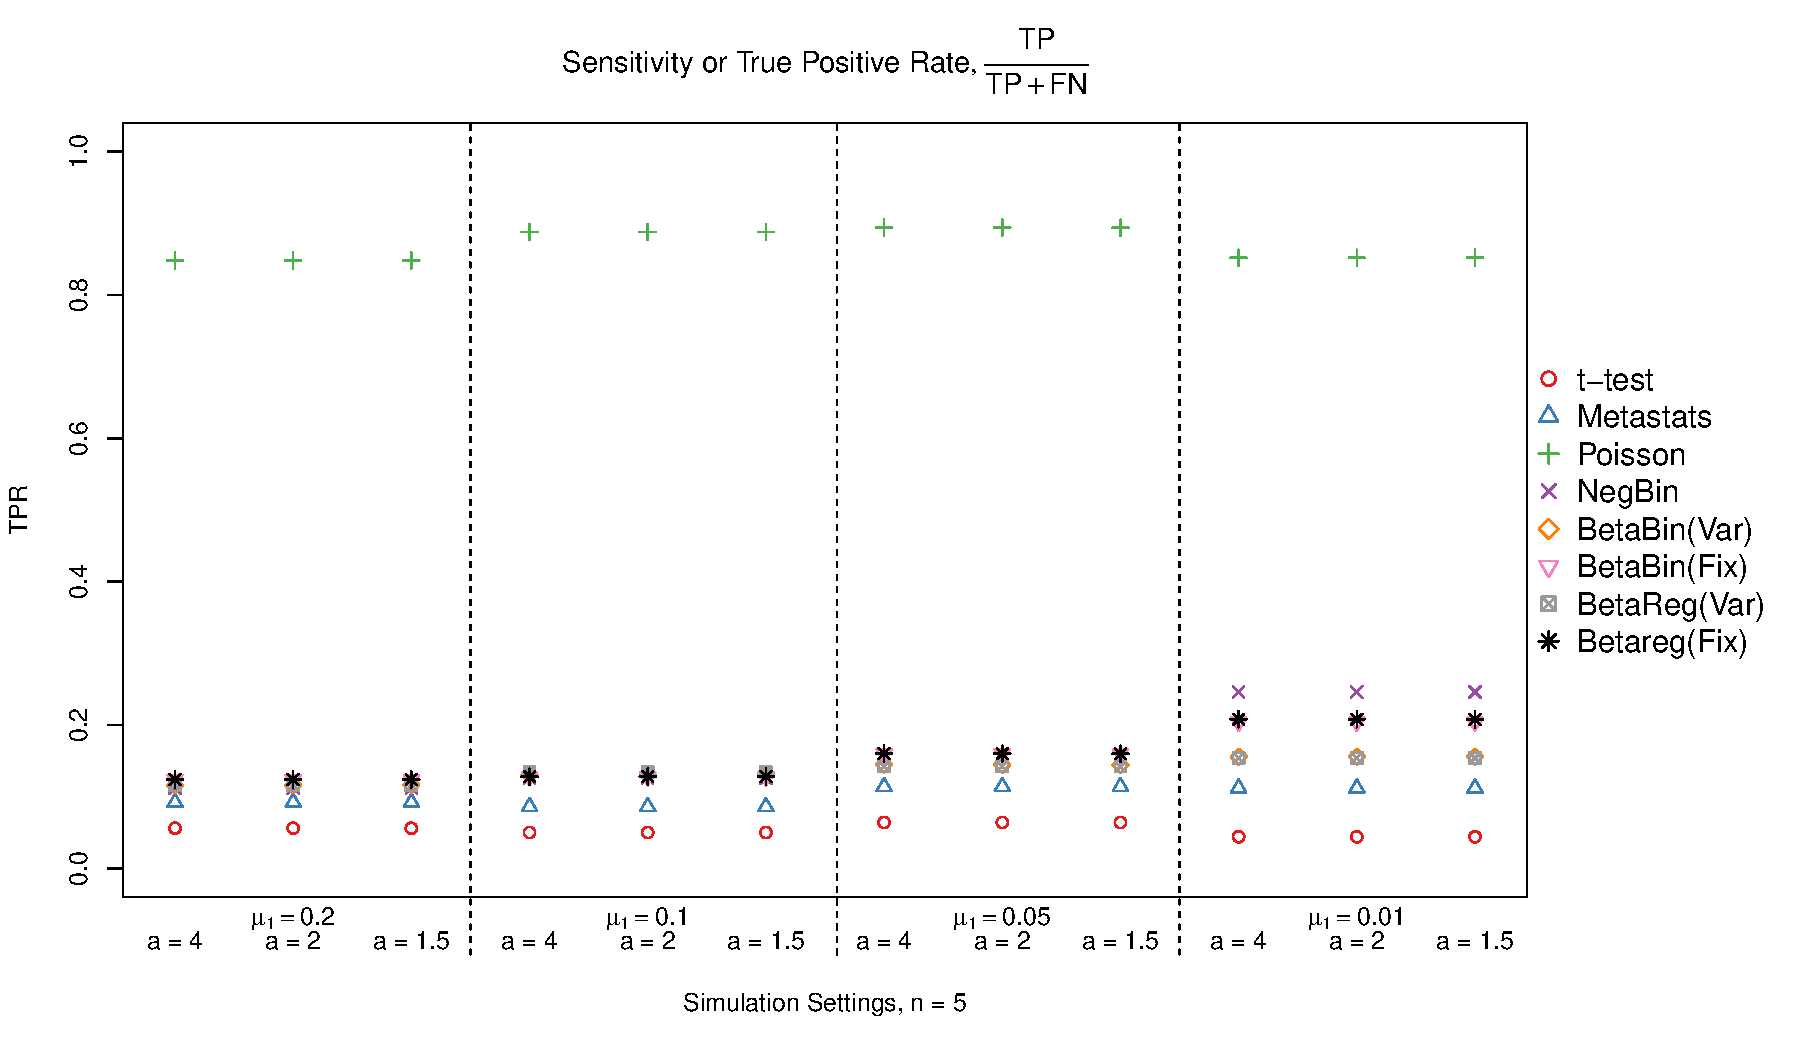
\includegraphics[width=\maxwidth]{figure/panelPlots1} 

}




{\centering 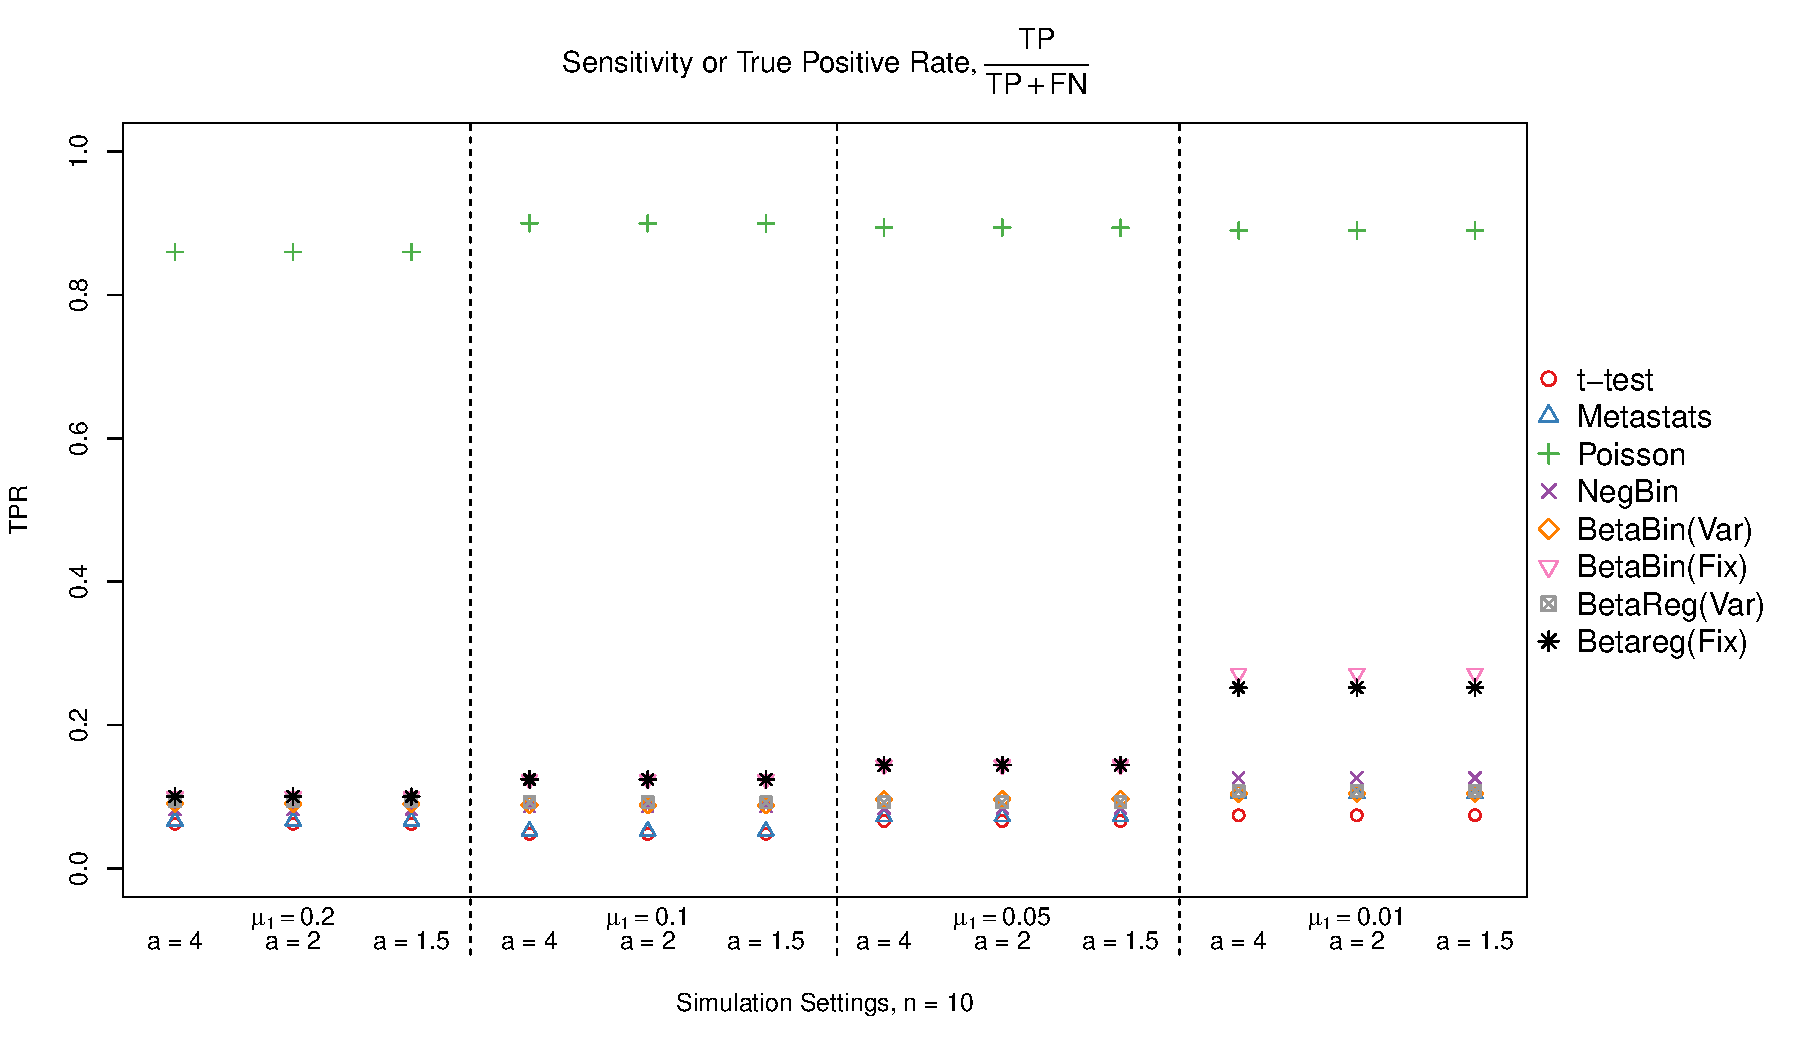
\includegraphics[width=\maxwidth]{figure/panelPlots2} 

}




{\centering 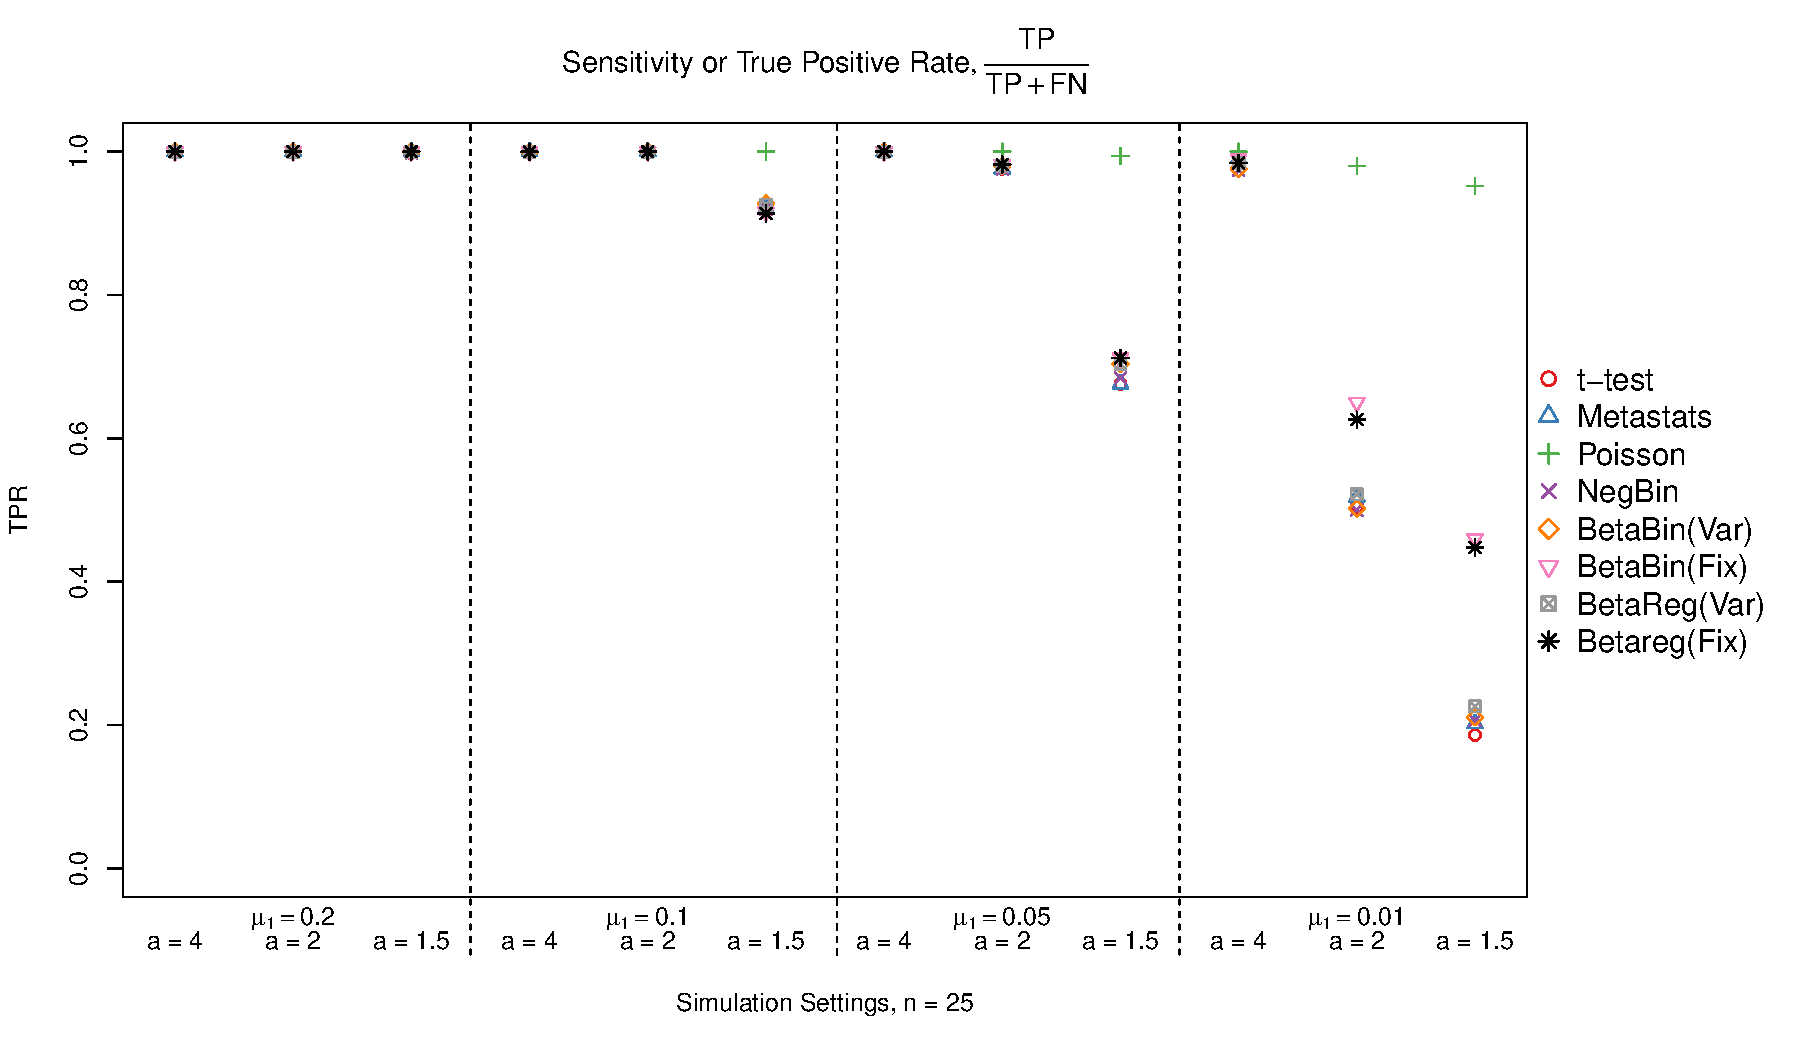
\includegraphics[width=\maxwidth]{figure/panelPlots3} 

}




{\centering 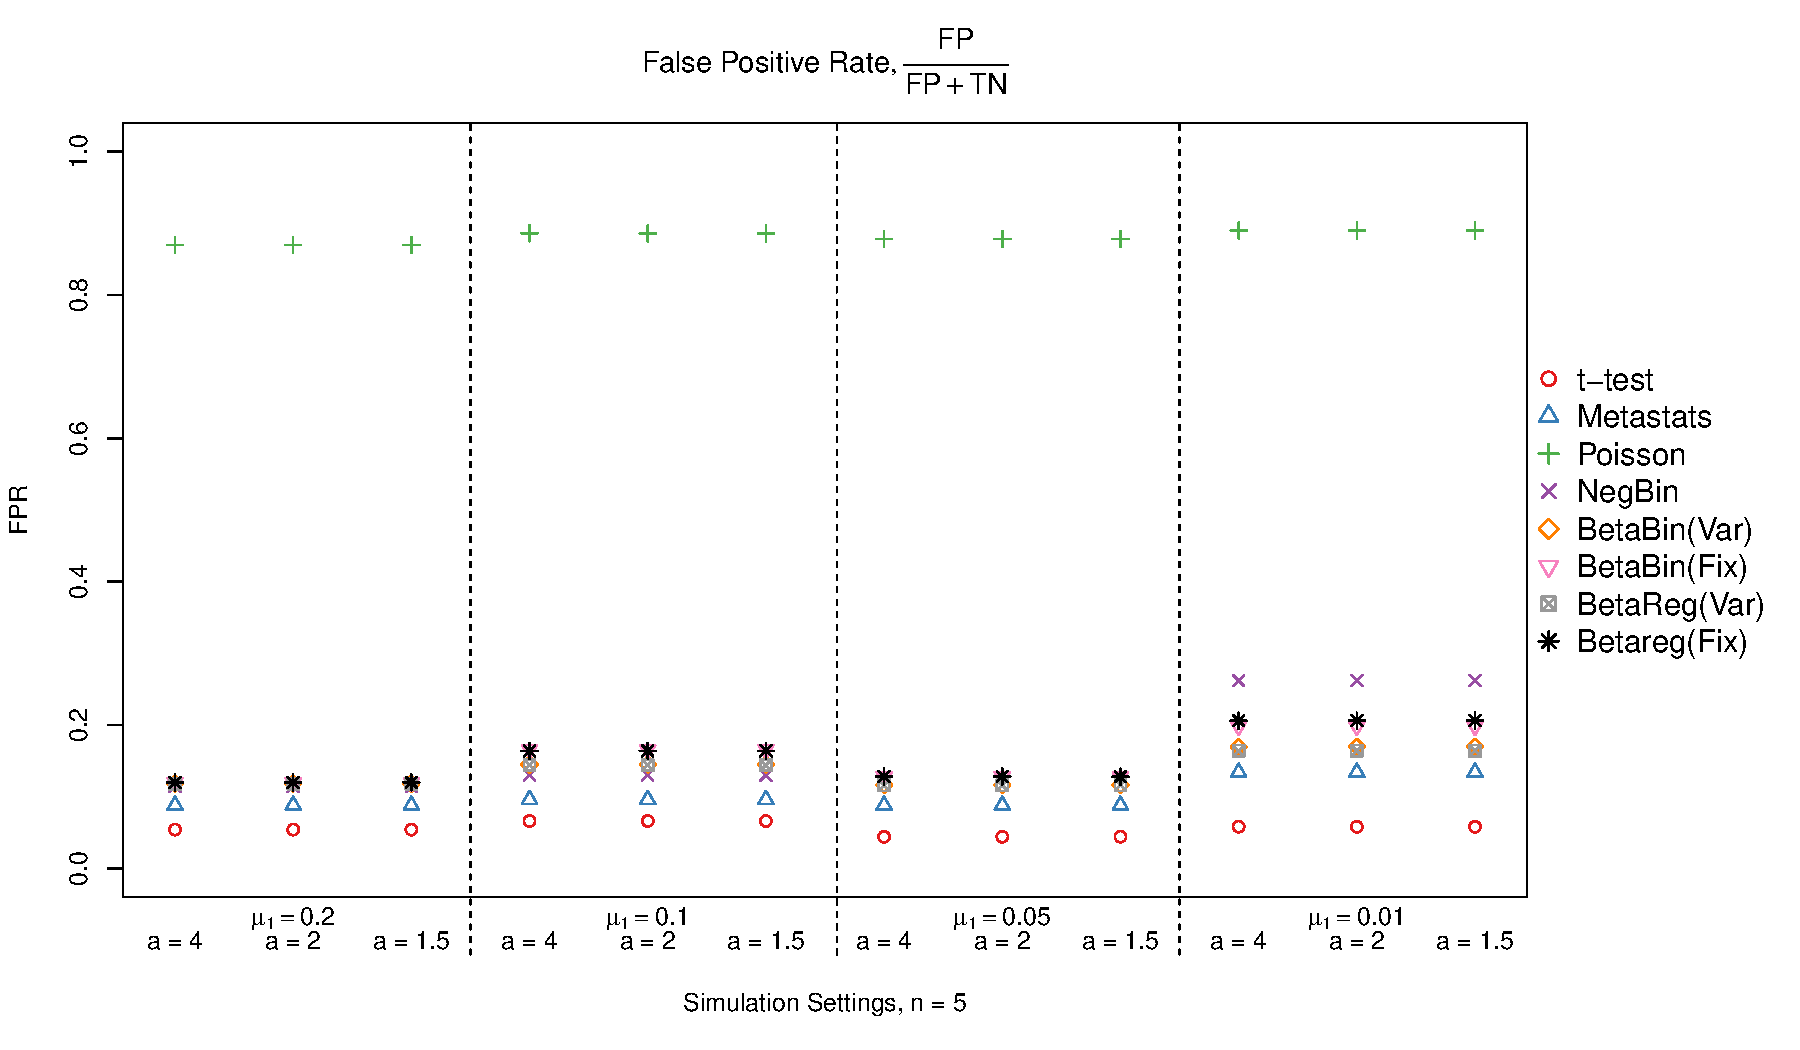
\includegraphics[width=\maxwidth]{figure/panelPlots4} 

}




{\centering 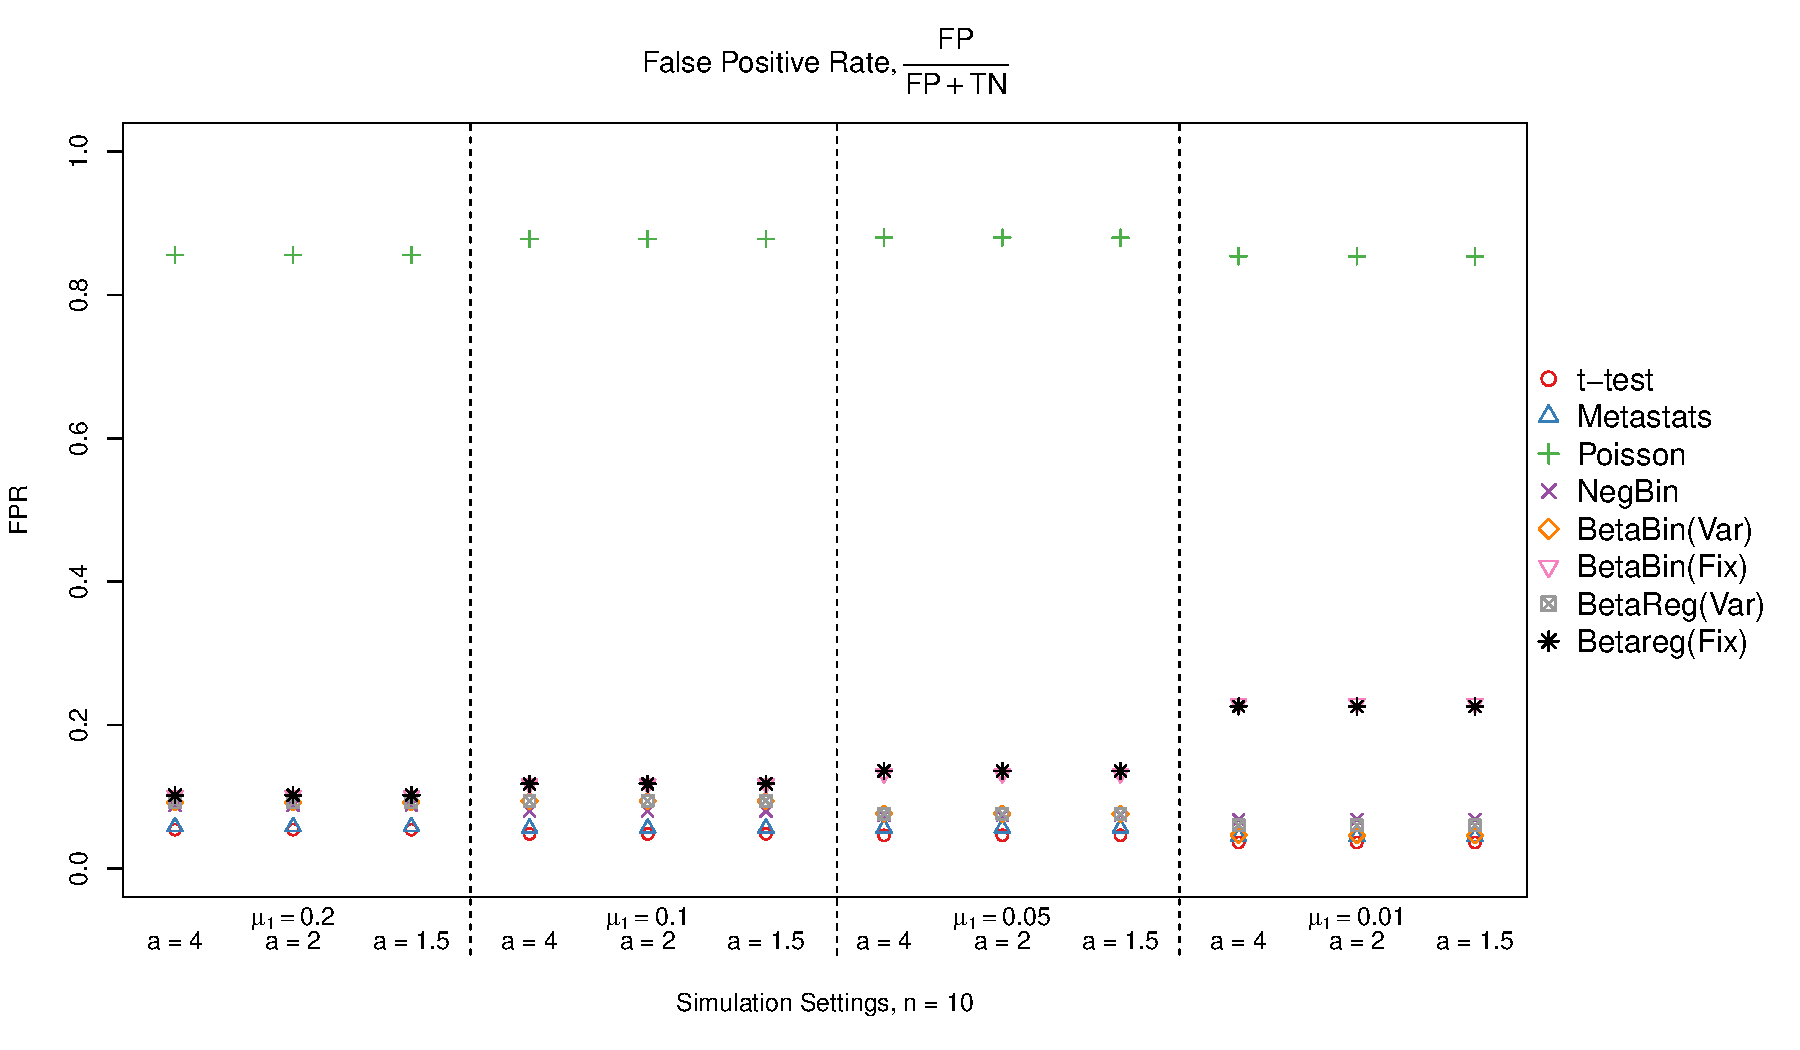
\includegraphics[width=\maxwidth]{figure/panelPlots5} 

}




{\centering 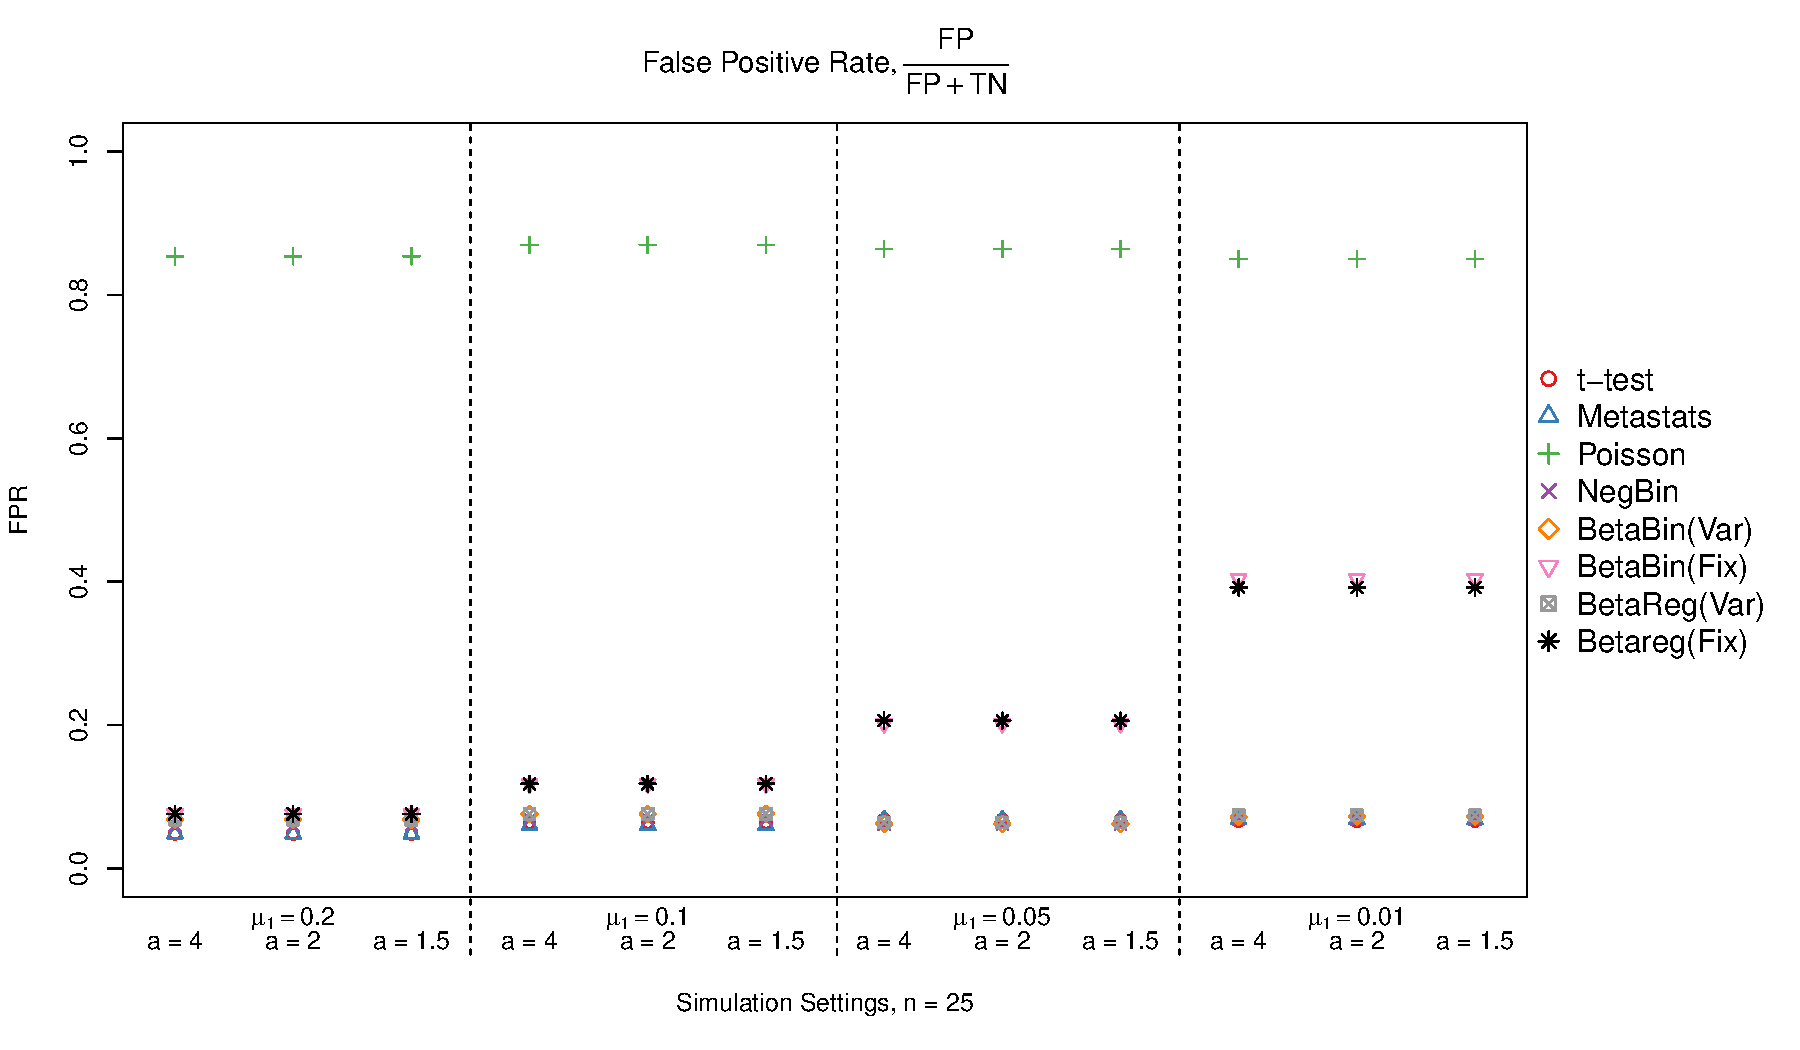
\includegraphics[width=\maxwidth]{figure/panelPlots6} 

}




{\centering 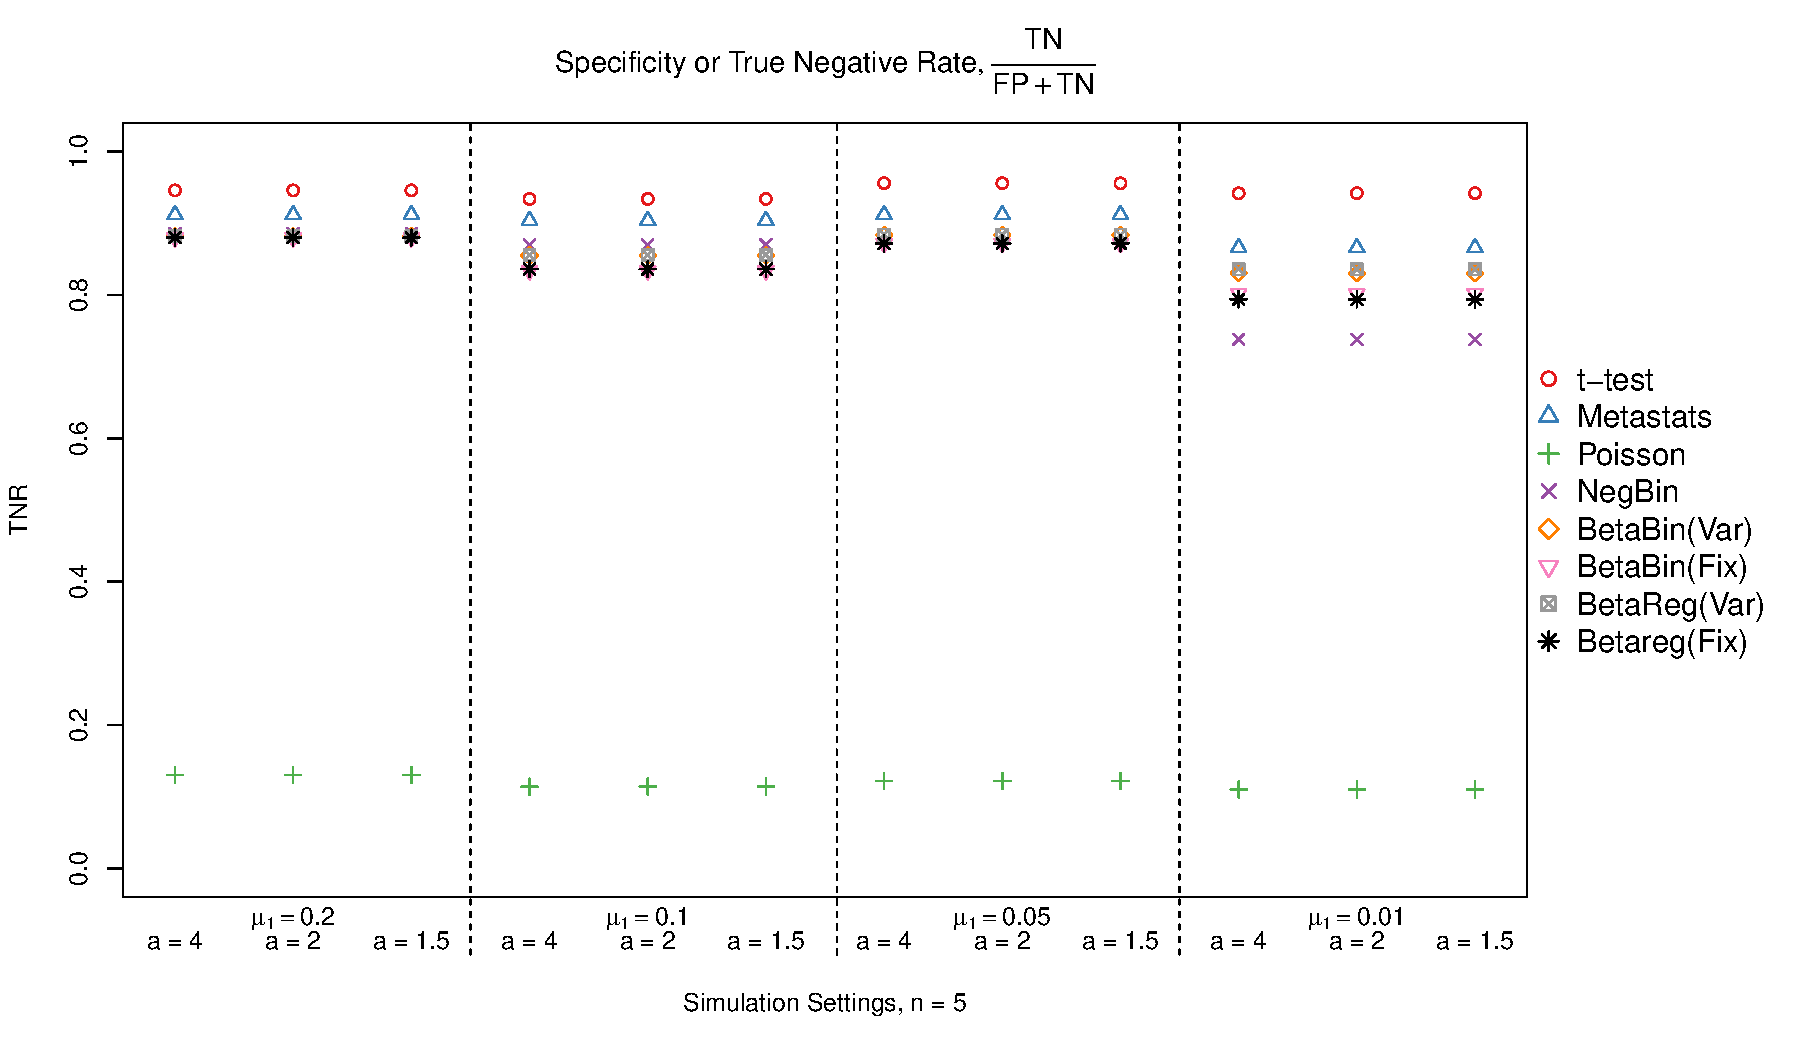
\includegraphics[width=\maxwidth]{figure/panelPlots7} 

}




{\centering 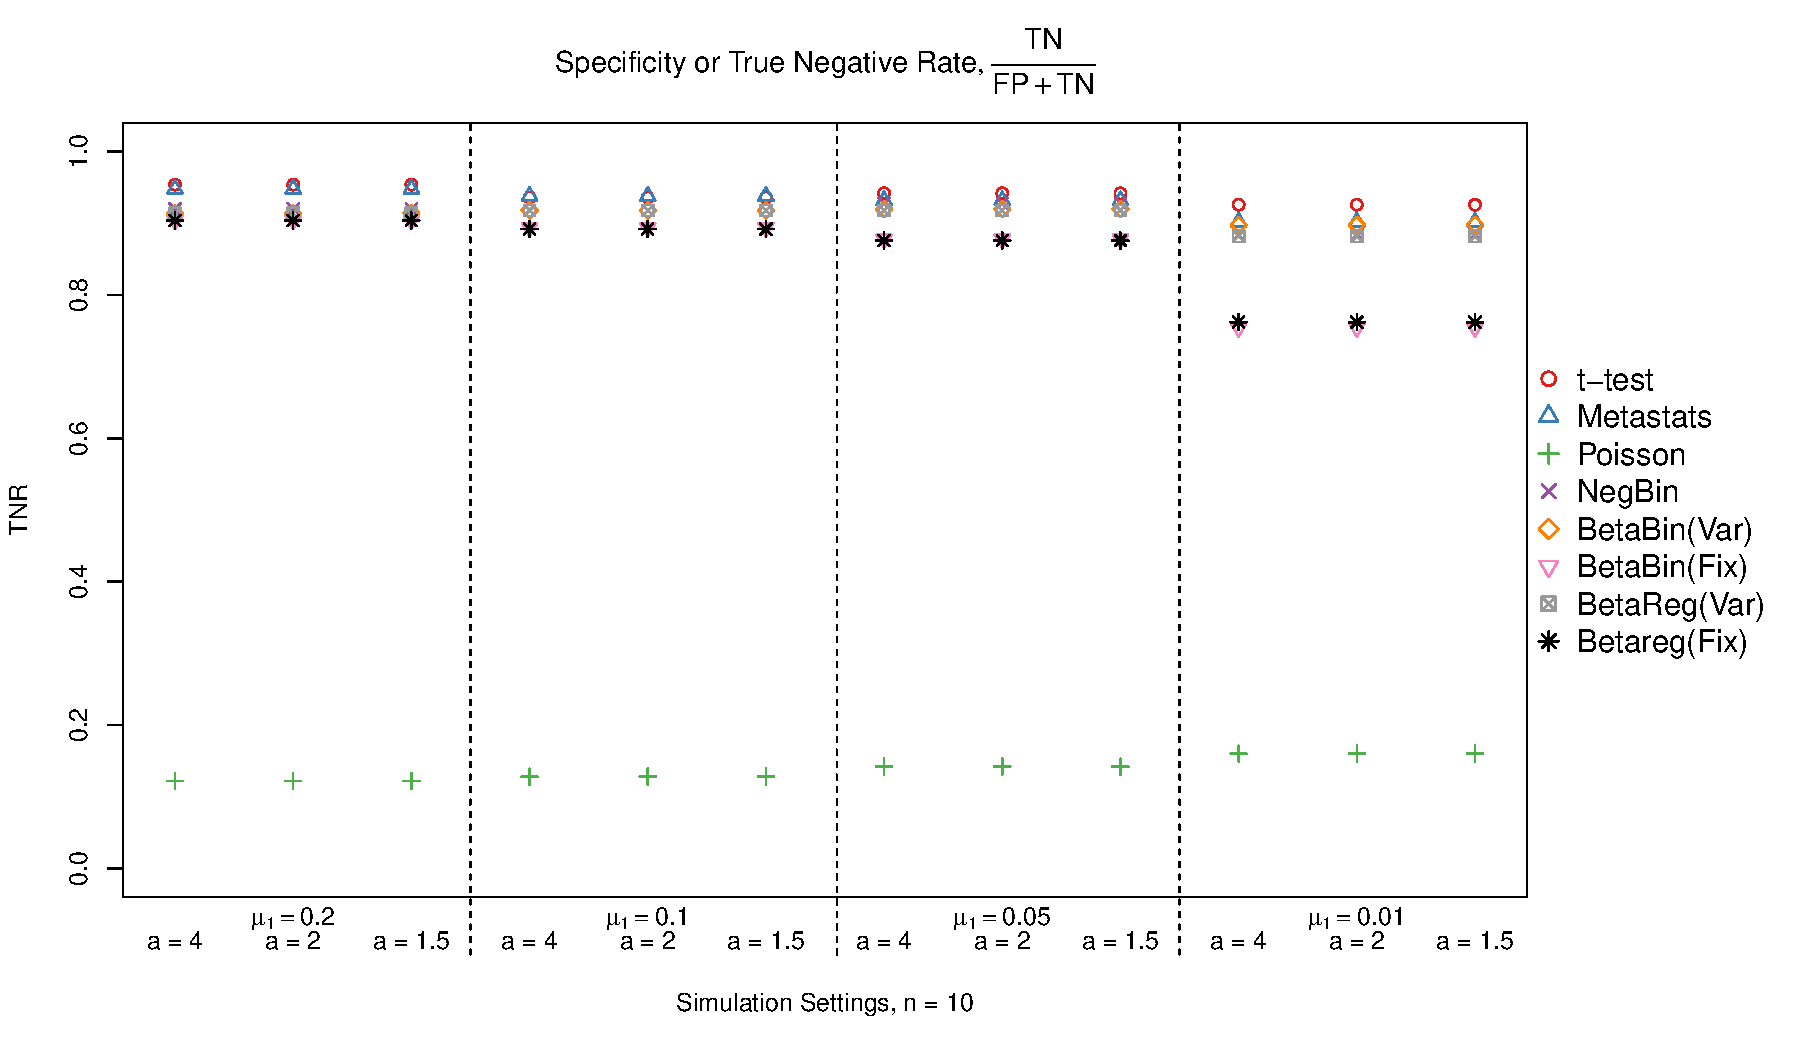
\includegraphics[width=\maxwidth]{figure/panelPlots8} 

}




{\centering 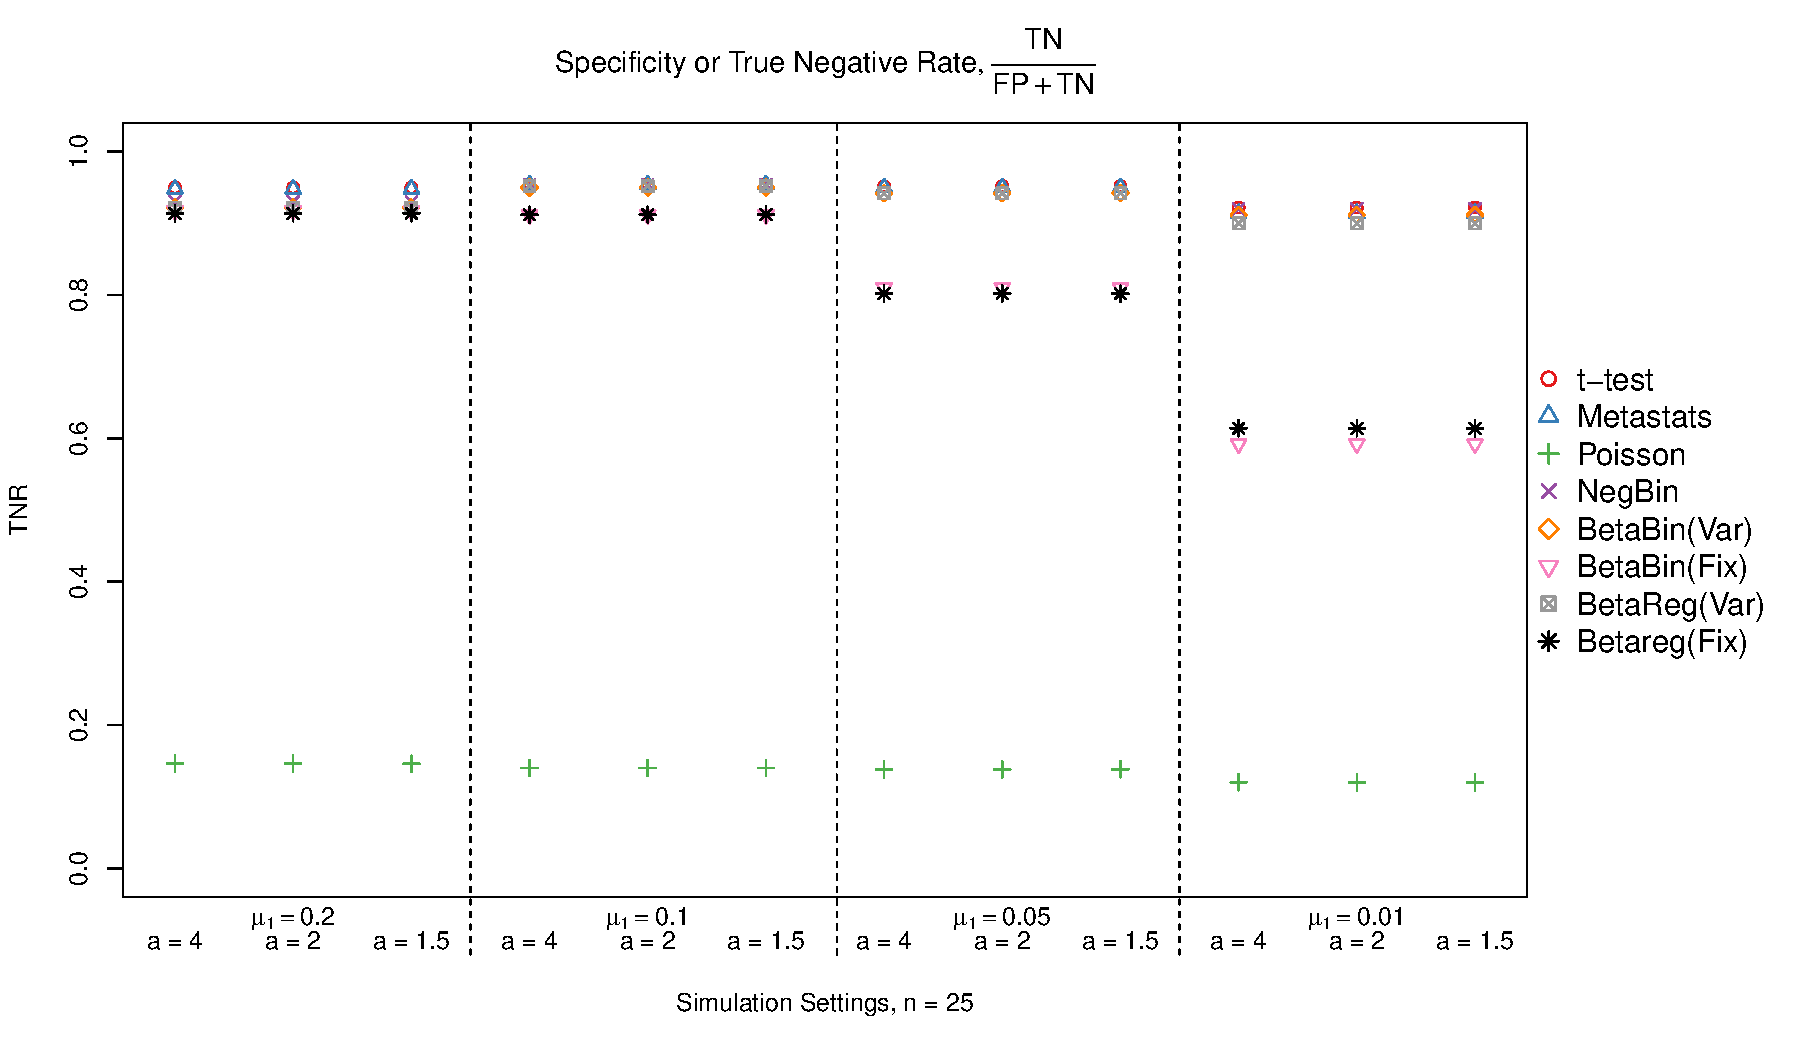
\includegraphics[width=\maxwidth]{figure/panelPlots9} 

}




{\centering 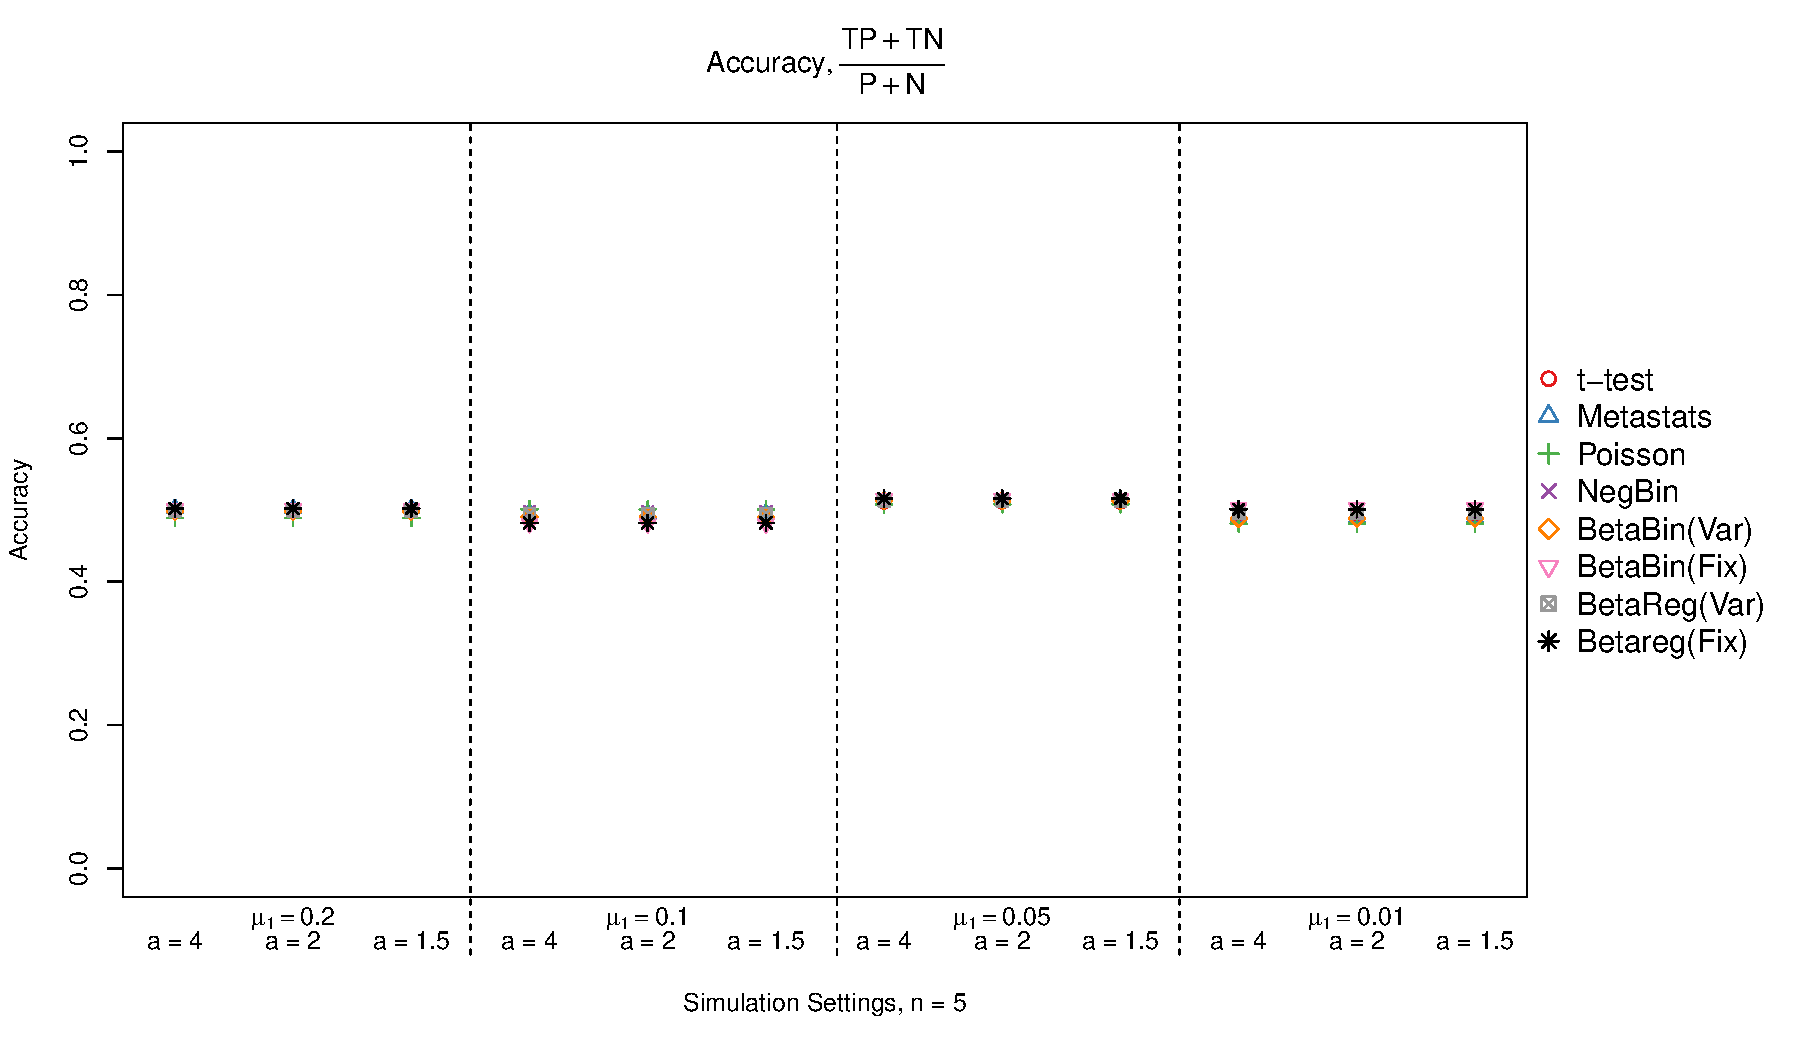
\includegraphics[width=\maxwidth]{figure/panelPlots10} 

}




{\centering 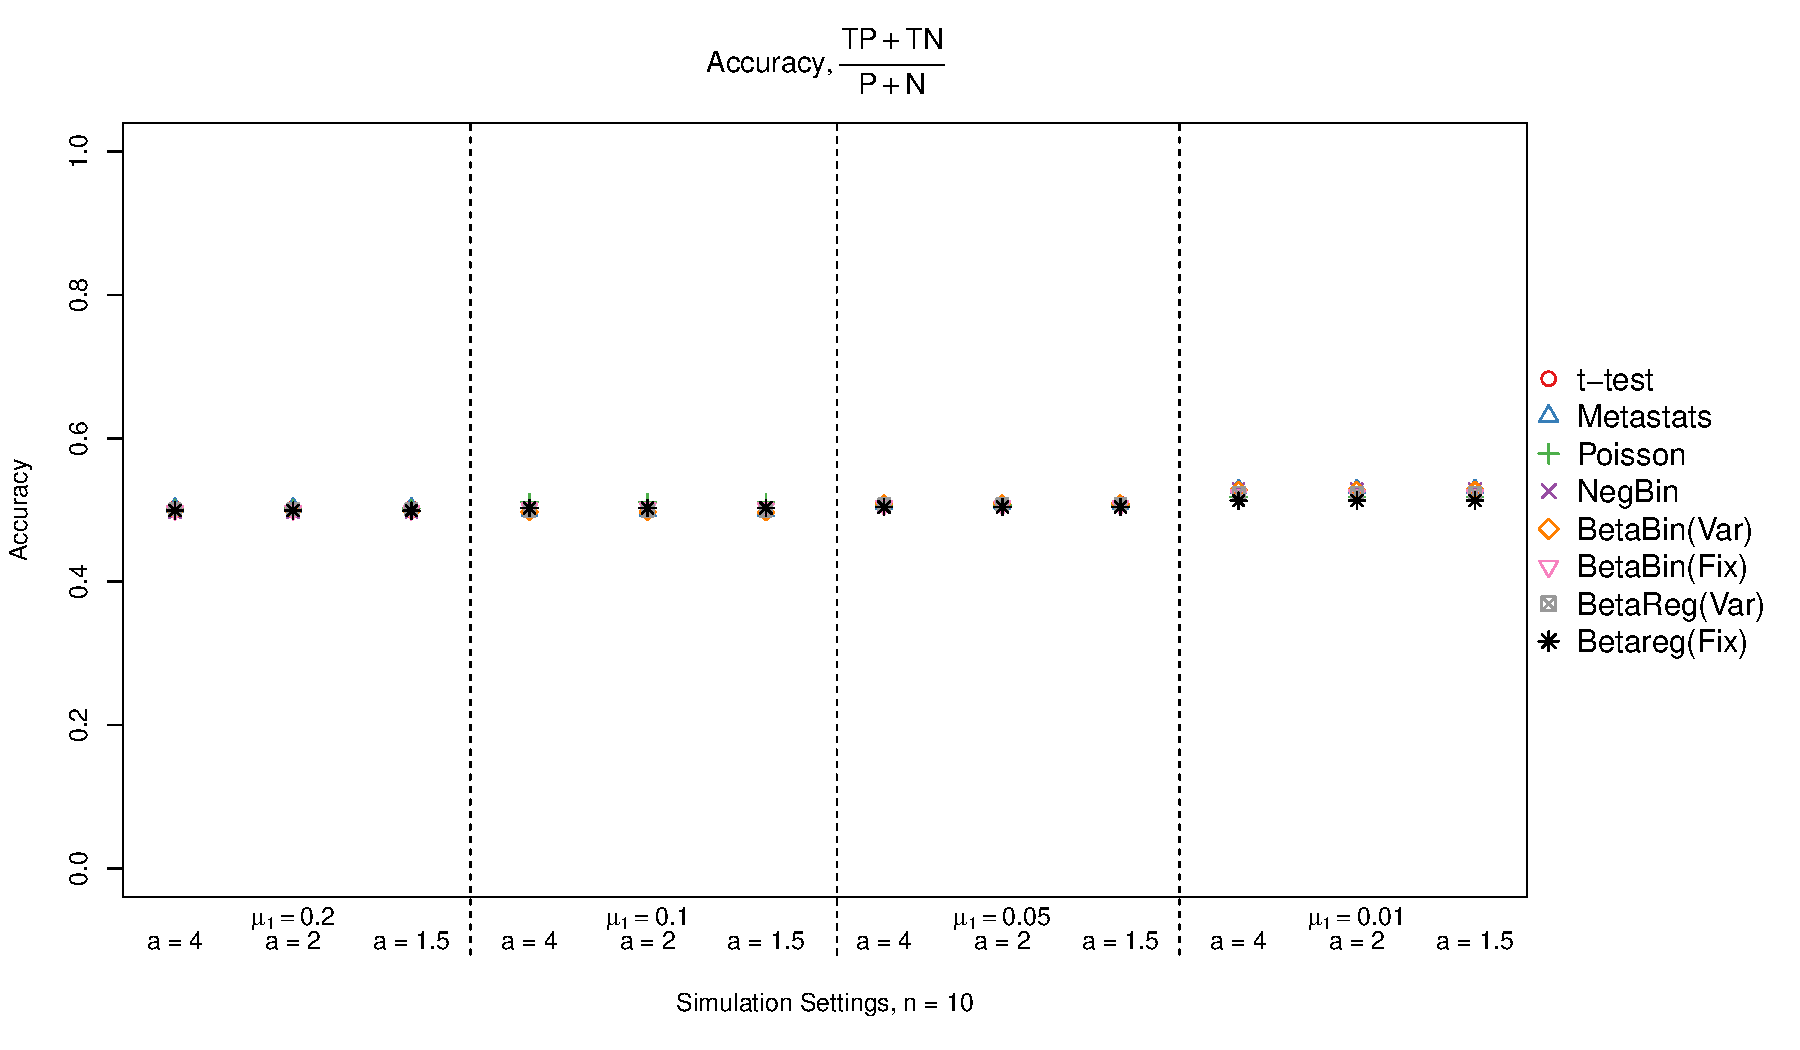
\includegraphics[width=\maxwidth]{figure/panelPlots11} 

}




{\centering 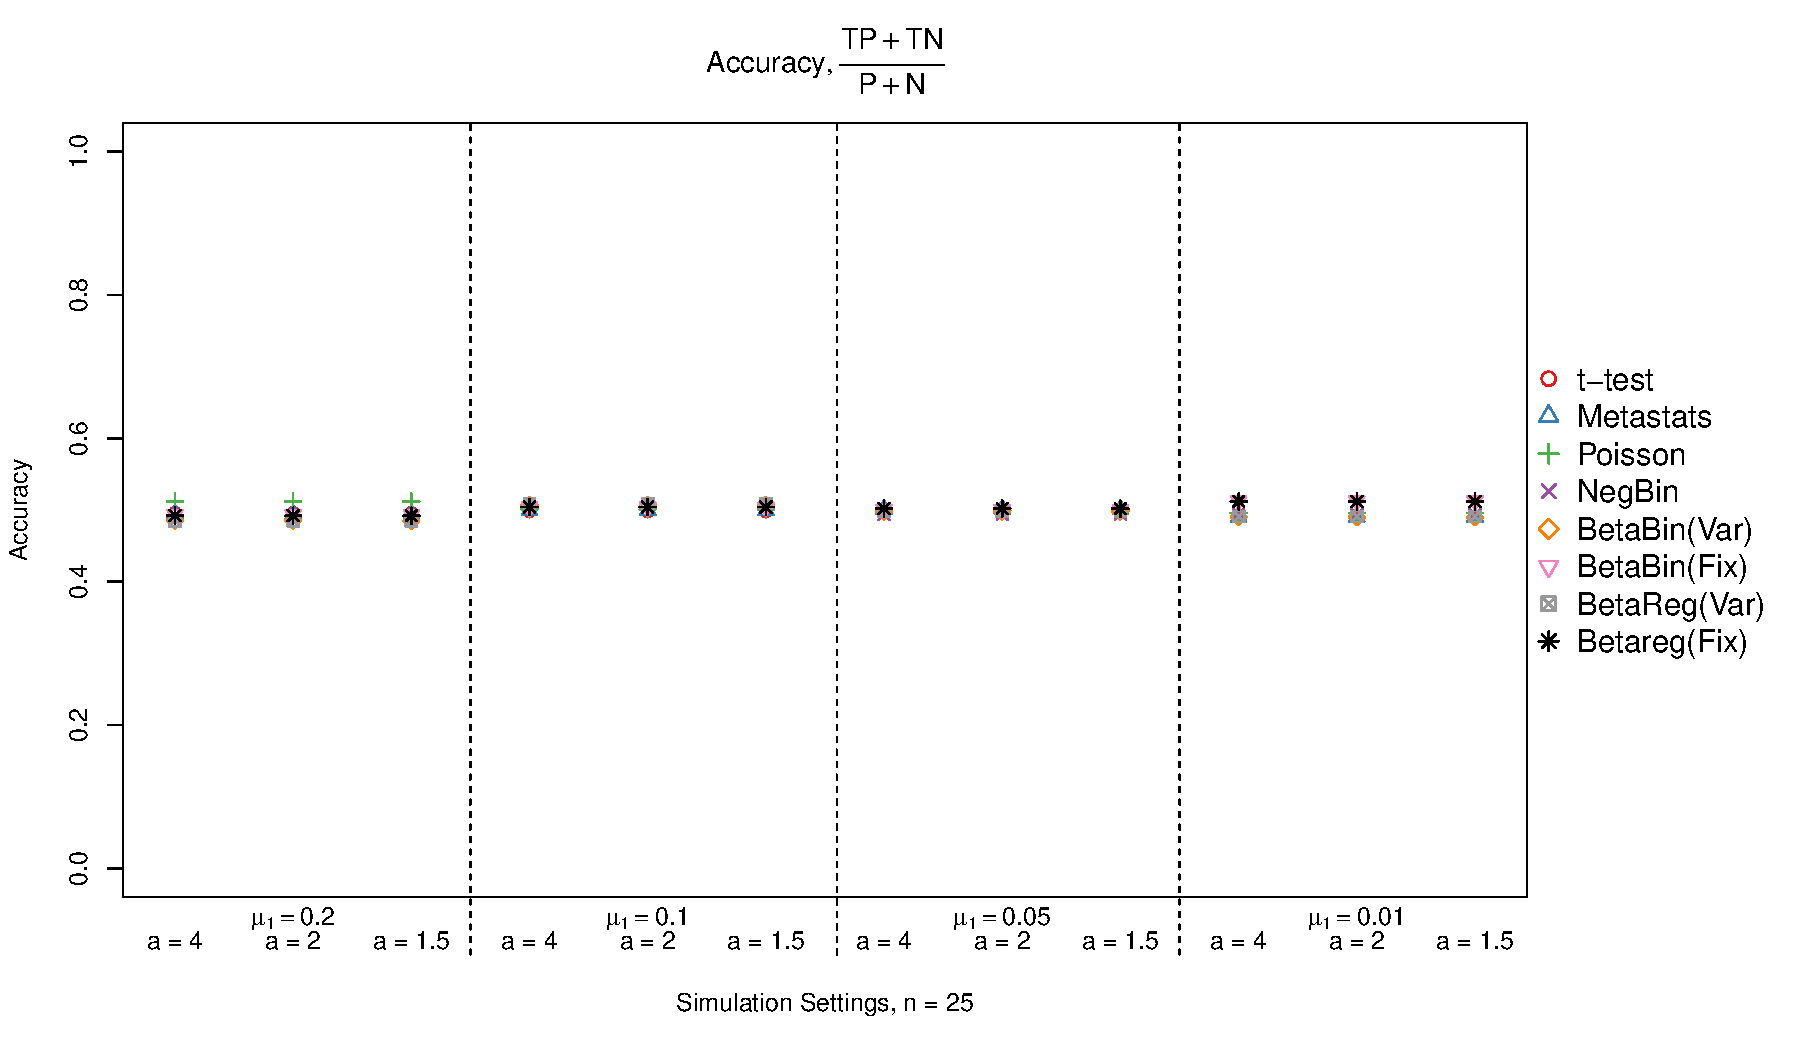
\includegraphics[width=\maxwidth]{figure/panelPlots12} 

}



\end{knitrout}


\end{document}







%%====Generic Templates====

%%----Figure Template----
% \begin{figure}[H]
%   \begin{center}
% <<figureName>>=
% print(plot(...))
% @
%     \caption{figure caption}
%   \end{center}
% \end{figure}

%%----Table Template----
% <<tableName, eval=TRUE, results='asis'>>=
% print(xtable(x,
%              digit=c(0),
%              caption="Caption",
%              label="tab:tableName"),
%       table.placement="H",include.rownames=TRUE, caption.placement="top")
% @
